\documentclass[12pt,a4paper]{article}
%\renewcommand{\familydefault}{\sfdefault}
\usepackage{amsmath}
\usepackage[a4paper, margin=0.6in]{geometry}
\usepackage{parskip}
\usepackage{tabulary}
\usepackage{float}
\usepackage{titling}
\usepackage{siunitx}
\usepackage{enumitem}

\usepackage[utf8]{inputenc}
\usepackage[english]{babel}
\usepackage{multicol}


\usepackage{graphicx}
\graphicspath{ {./result_images/} }

\setlength{\droptitle}{-3em}

\title{COMP4421 Assignment 1}
\author{MOHAMAD, Randitya Setyawan\\20316273\\ \texttt{rsmohamad@ust.hk}}


\begin{document}
	\maketitle
	
	\section{Exercises}
	\begin{enumerate}
		\item \textbf{Fourier Transform}
		\begin{enumerate}
			\item The significant increase across the vertical and horizontal axes in the frequency domain is caused by the abrupt changes in intensity between the image and the black padding. The vertical and horizontal boundary between the image and the black padding have a large gradient with respect to the y and x axes respectively. These large changes contribute to the vertical and horizontal axes in the frequency domain representation.
			\item The significant increase in the low frequency region is caused by the black padding which does not change intensity accross a large area. This contributes to the low frequency components in the frequency domain representation.
		\end{enumerate}
	\end{enumerate}

	\pagebreak
	\section{Programming Tasks}
	\begin{enumerate}
		\item \textbf{Spatial Linear Filtering}
		\begin{enumerate}
			\begin{multicols}{2}
			\item Average filter \\
			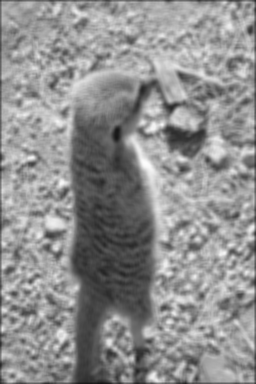
\includegraphics[scale=0.75]{task1/img_ave.png}
			\item Sobel X \\
			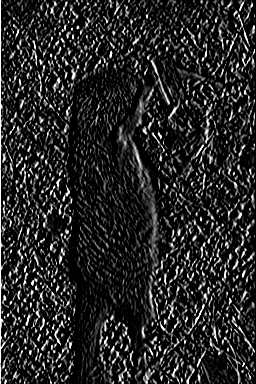
\includegraphics[scale=0.75]{task1/img_dx.png}
			\item Sobel Y \\
			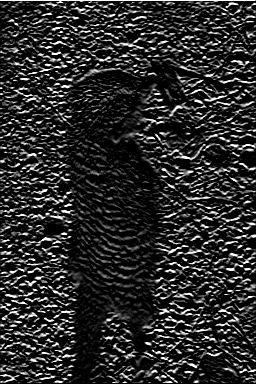
\includegraphics[scale=0.75]{task1/img_dy.png}
			\item Laplacian filter \\
			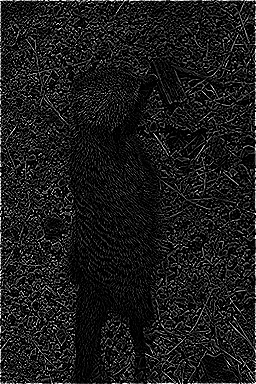
\includegraphics[scale=0.75]{task1/img_sharpen.png}
			\end{multicols}
		\end{enumerate}

		\pagebreak
		\item \textbf{Spatial Non-linear Filtering}
		\begin{enumerate}
			\begin{multicols}{2}
			\item Gaussian noise \\
			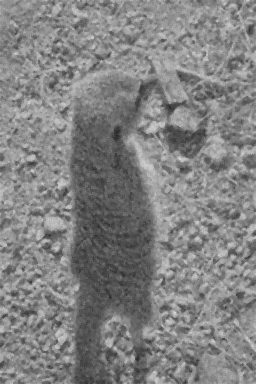
\includegraphics[scale=0.75]{task2/med_gaussian.png}
			
			\item Salt and pepper noise \\
			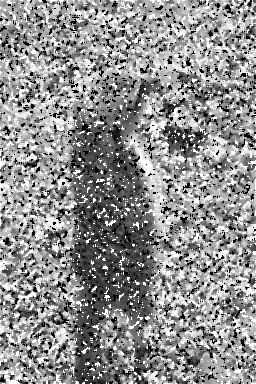
\includegraphics[scale=0.75]{task2/med_sp.png}
			\end{multicols}
		\end{enumerate}

		\item \textbf{Discrete Fourier Transform}
		\begin{enumerate}
			\begin{multicols}{2}
			\item Frequency spectrum \\ 
			
\includegraphics[scale=0.75]{task3/dft_spectrum.png}
			\item Inverse DFT real component \\
			
\includegraphics[scale=0.75]{task3/idft_real.png}
			\end{multicols}
		\end{enumerate}

		\pagebreak
		\item \textbf{Filtering in the Frequency Domain}
		\begin{enumerate}
			\begin{multicols}{2}
			\item Average filter \\
			
\includegraphics[scale=0.75]{task4/img_ave_freq.png}
			\item Laplacian filter \\
			
\includegraphics[scale=0.75]{task4/img_sharpen_freq.png}
			\end{multicols}
		\end{enumerate}

		\item \textbf{High-Frequency Emphasis} \textit{(a = 0.1, b = 0.9)}
		\begin{enumerate}
			\begin{multicols}{2}
			\item Butterworth \\
			
\includegraphics[scale=0.75]{task5/butter.png}
			\item Gaussian \\
			
\includegraphics[scale=0.75]{task5/gaussian.png}
			\end{multicols}
		\end{enumerate}
	\end{enumerate}
		
\end{document}

